\documentclass[12pt,a4paper]{extarticle}
\usepackage[utf8]{inputenc}
\usepackage[T5]{fontenc}
\usepackage{geometry}
\geometry{a4paper, left=1.5cm, right=1cm, top=1.5cm, bottom=1.5cm, headheight=20pt, headsep=15pt, footskip=28pt}
\usepackage{enumitem}
\usepackage{amsmath}
\usepackage{amssymb}
\usepackage{diagbox}
\usepackage{colortbl} % Sửa lỗi \arrayrulecolor
\usepackage{array}    % Hỗ trợ định dạng cột m{2cm}
\usepackage[most]{tcolorbox}
\newcommand{\khongxacdinh}{\text{KXĐ}}
\newcommand{\blackbox}[1]{\texorpdfstring{\fcolorbox{black}{black}{\textcolor{white}{#1}}}{#1}}
\usepackage{tikz}
\definecolor{bookblue}{RGB}{58,90,172}
\definecolor{book}{RGB}{58,90,172}
\definecolor{myblue}{RGB}{200,40,40}
\newcommand{\bluecheck}{\textcolor{myblue}{\checkmark}}
\newtcolorbox{formulaBox}{colback=gray!5,colframe=bookblue,boxrule=0.8pt,arc=2mm}
\newtcolorbox{notebox}{colback=blue!3,colframe=myblue,boxrule=0.8pt,arc=2mm}
\usetikzlibrary{patterns, patterns.meta} % Thêm patterns.meta vào đây
% Gọi package nằm trong thư mục con template
\usepackage{../template/mngocbox}

\begin{document}

% Sử dụng ngoặc vuông [...] để thay đổi linh hoạt các thông số
\makeheadbox[headerright={Chương 4},chude={Bài 3},tieude={Ứng dụng tích phân},dinhdang={Giải tích},lop={12 },gv={Nguyễn Lê Minh Ngọc}]
\vspace{2em}
\section*{\color{myblue}{1. ỨNG DỤNG TÍCH PHÂN ĐỂ TÍNH DIỆN TÍCH HÌNH PHẲNG}}
\subsection*{\color{myblue}{a) Hình phẳng giới hạn bởi một đồ thị hàm số, trục hoành và hai đường thẳng $x=a, x=b$}}
\begin{tcolorbox}[colback=lightblue, colframe=myblue, arc=2mm]
Diện tích $S$ của hình phẳng giới hạn bởi đồ thị hàm số $f(x)$ liên tục, trục hoành và hai đường thẳng $x = a$, $x = b$ ($a < b$), được tính bằng công thức:
\[
S = \int_{a}^{b} |f(x)| \, \mathrm{d}x
\]
\end{tcolorbox}
\subsection*{\color{myblue}{b) Hình phẳng giới hạn bởi hai đồ thị hàm số và hai đường thẳng $x=a, x=b$}}
\begin{tcolorbox}[colback=lightblue, colframe=myblue, arc=2mm]
Diện tích $S$ của hình phẳng giới hạn bởi đồ thị của hai hàm số $f(x)$, $g(x)$ liên tục trên đoạn $[a; b]$ và hai đường thẳng $x = a$, $x = b$, được tính bằng công thức:
\[
S = \int_{a}^{b} |f(x) - g(x)| \, \mathrm{d}x
\]
\end{tcolorbox}
\vspace{0.5cm}
\noindent \textbf{\color{myblue}{\textit{Chú ý:}}} Nếu hiệu $f(x) - g(x)$ không đổi dấu trên đoạn $[a; b]$ thì:
\[
\int_{a}^{b} |f(x) - g(x)| \, \mathrm{d}x = \left| \int_{a}^{b} [f(x) - g(x)] \, \mathrm{d}x \right|
\]

\subsection*{\color{myblue}{c) Thặng dư tiêu dùng}}
\begin{tcolorbox}[colback=lightblue, colframe=myblue, arc=2mm]
Ta biết rằng hàm cầu liên quan đến giá $p$ của một sản phẩm với nhu cầu của người tiêu dùng, hàm cung liên quan đến giá $p$ của sản phẩm với mức độ sẵn sàng cung cấp sản phẩm của nhà sản xuất. Điểm cắt nhau $(x_0; p_0)$ của đồ thị hàm cầu $p = D(x)$ và đồ thị hàm cung $p = S(x)$ được gọi là \textbf{điểm cân bằng}.
\vspace{0.2cm}
Các nhà kinh tế gọi diện tích của hình giới hạn bởi đồ thị hàm cầu, đường ngang $p = p_0$ và đường thẳng đứng $x = 0$ là \textit{thặng dư tiêu dùng}. Tương tự, diện tích của hình phẳng giới hạn bởi đồ thị của hàm cung, đường nằm ngang $p = p_0$ và đường thẳng đứng $x = 0$ được gọi là \textit{thặng dư sản xuất}, như trong hình vẽ.
\end{tcolorbox}
\vspace{0.5cm}
% ==================== HÌNH VẼ TIKZ ====================
\begin{center}
\begin{tikzpicture}[scale=1.2, >=stealth]
  % Định nghĩa các điểm
  \coordinate (O) at (0,0);
  \coordinate (X0) at (3,0);
  \coordinate (P0) at (0,2.5);
  \coordinate (E) at (3,2.5);
  % 1. Miền thặng dư tiêu dùng (Màu xanh lam nhạt)
  \fill[cyan!35] (0,2.5) -- plot[domain=0:3, smooth] (\x, {4.5 - 0.4*\x - 0.08*\x*\x}) -- (0,2.5) -- cycle;
  % 2. Miền thặng dư sản xuất (Màu hồng/đỏ nhạt)
  \fill[pink!80!red] (0,1.2) -- (0,2.5) -- (3,2.5) -- plot[domain=3:0, smooth] (\x, {1.2 + 0.2*\x + 0.0778*\x*\x}) -- cycle;
  % 3. Vẽ đường cong Hàm cầu (Demand curve)
  \draw[line width=1.3pt, magenta] plot[domain=0:4.1, smooth] (\x, {4.5 - 0.4*\x - 0.08*\x*\x});
  \node[above right, font=\small\bfseries] at (0.2, 4.1) {Hàm cầu};
  % 4. Vẽ đường cong Hàm cung (Supply curve)
  \draw[line width=1.3pt, magenta] plot[domain=0:4.1, smooth] (\x, {1.2 + 0.2*\x + 0.0778*\x*\x});
  \node[below right, font=\small\bfseries] at (0.5, 1.1) {Hàm cung};
  % 5. Các đường nét đứt nét nối điểm cân bằng
  \draw[dashed, line width=0.8pt] (0,2.5) -- (3,2.5) -- (3,0);
  % 6. Các trục tọa độ
  \draw[->, line width=1pt] (-0.3,0) -- (4.8,0) node[below] {$x$};
  \draw[->, line width=1pt] (0,-0.3) -- (0,4.8) node[left] {$p$};
  % 7. Nhãn các trục
  \node[below left] at (O) {$O$};
  \node[left] at (P0) {$p_0$};
  \node[below] at (X0) {$x_0$};
  % 8. Điểm cân bằng
  \fill (E) circle (2.2pt);
  \node[above, font=\small\bfseries] at (3.3, 2.6) {Điểm cân bằng};
  \node[right, font=\small] at (3.5, 2.3) {$(x_0; p_0)$};
  % 9. Chú thích trong miền tô màu
  \node[align=center, font=\scriptsize\bfseries] at (1.0, 3.1) {Thặng dư\\tiêu dùng};
  \node[align=center, font=\scriptsize\bfseries] at (1.0, 1.8) {Thặng dư\\sản xuất};
\end{tikzpicture}
\end{center}
% ======================================================
\vspace{0.3cm}

\section*{\color{myblue}{1. ỨNG DỤNG TÍCH PHÂN ĐỂ TÍNH THỂ TÍCH VẬT THỂ}}
\subsection*{\color{myblue}{a) Tính thể tích của vật thể}}
\begin{tcolorbox}[colback=lightblue, colframe=myblue, arc=2mm]
Cho một vật thể trong không gian $Oxyz$. Gọi $\beta$ là phần vật thể giới hạn bởi hai mặt phẳng vuông góc với trục $Ox$ tại các điểm có hoành độ $x = a, x = b$. Một mặt phẳng vuông góc với trục $Ox$ tại điểm có hoành độ là $x$ cắt vật thể theo mặt cắt có diện tích là $S(x)$. Giả sử $S(x)$ là hàm số liên tục trên đoạn $[a; b]$. Khi đó, thể tích $V$ của phần vật thể $\beta$ được tính bởi công thức:
\[
V = \int_{a}^{b} S(x) \, \mathrm{d}x.
\]
\end{tcolorbox}
\vspace{0.4cm}
% ==================== HÌNH VẼ TIKZ VẬT THỂ (SECTION A) ====================
\begin{center}
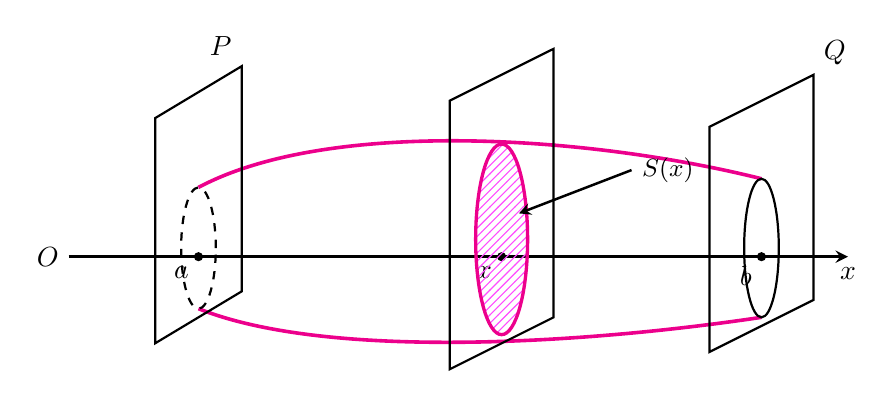
\begin{tikzpicture}[scale=1.1, >=stealth]
  % Axis Ox
  \draw[->, line width=1pt] (-0.5,0) -- (8.5,0) node[below] {$x$};
  \node[left] at (-0.5,0) {$O$};
  
  % Points on axis
  \fill (1,0) circle (1.5pt) node[below left] {$a$};
  \fill (4.5,0) circle (1.5pt) node[below left] {$x$};
  \fill (7.5,0) circle (1.5pt) node[below left] {$b$};
  % Outer boundary curves of the 3D solid
  \draw[line width=1.3pt, magenta] (1,0.8) .. controls (2.5, 1.6) and (5.5, 1.4) .. (7.5, 0.9);
  \draw[line width=1.3pt, magenta] (1,-0.6) .. controls (2.5, -1.2) and (5.5, -1.0) .. (7.5, -0.7);
  % Plane P at x = a
  \draw[line width=0.8pt] (0.5, -1.0) -- (0.5, 1.6) -- (1.5, 2.2) node[above left] {$P$} -- (1.5, -0.4) -- cycle;
  \draw[line width=0.8pt, dashed] (1, 0.1) ellipse (0.2cm and 0.7cm);
  % Slice at x with area S(x)
  \draw[line width=0.8pt] (3.9, -1.3) -- (3.9, 1.8) -- (5.1, 2.4) -- (5.1, -0.7) -- cycle;
  \fill[pattern=north east lines, pattern color=magenta!70] (4.5, 0.2) ellipse (0.3cm and 1.1cm);
  \draw[line width=1.2pt, magenta] (4.5, 0.2) ellipse (0.3cm and 1.1cm);
  
  % Pointer to S(x)
  \draw[->, line width=0.9pt] (6.0, 1.0) node[right, font=\bfseries\small] {$S(x)$} -- (4.7, 0.5);
  % Plane Q at x = b
  \draw[line width=0.8pt] (6.9, -1.1) -- (6.9, 1.5) -- (8.1, 2.1) node[above right] {$Q$} -- (8.1, -0.5) -- cycle;
  \draw[line width=0.8pt] (7.5, 0.1) ellipse (0.2cm and 0.8cm);
\end{tikzpicture}
\end{center}
% =========================================================================
\vspace{0.3cm}
\noindent \textbf{\color{myblue}{\textit{Chú ý:}}} Bằng ứng dụng của tích phân, người ta chứng minh được thể tích của khối chóp bất kì bằng $\frac{1}{3}$ diện tích mặt đáy nhân với chiều cao của nó.
\vspace{0.6cm}
\subsection*{\color{myblue}{b) Thể tích khối tròn xoay}}
\begin{tcolorbox}[colback=lightblue, colframe=myblue, arc=2mm]
Cho hàm số $f(x)$ liên tục, không âm trên đoạn $[a; b]$.
\vspace{0.2cm}
Khi quay hình phẳng giới hạn bởi đồ thị hàm số $y = f(x)$, trục hoành và hai đường thẳng $x = a, x = b$ xung quanh trục hoành, ta được hình khối gọi là một \textbf{khối tròn xoay}.
\vspace{0.2cm}
Khi cắt khối tròn xoay đó bởi một mặt phẳng vuông góc với trục $Ox$ tại điểm $x \in [a; b]$ được một hình tròn có bán kính $f(x)$.
\vspace{0.2cm}
Thể tích của khối tròn xoay này là:
\[
V = \pi \int_{a}^{b} f^2(x) \, \mathrm{d}x.
\]
\end{tcolorbox}
\subsection*{\color{myblue}{c) Ứng dụng tích phân trong toán chuyển động}}
\begin{tcolorbox}[colback=lightblue, colframe=myblue, arc=2mm]
\noindent Gia tốc là đạo hàm của vận tốc:
\[
a(t) = v'(t) \Rightarrow v(t) = \int a(t) \, \mathrm{d}t
\]
\noindent Vận tốc là đạo hàm của quãng đường:
\[
v(t) = s'(t) \Rightarrow s(t) = \int v(t) \, \mathrm{d}t \quad \text{nếu } v(t) \ge 0 \;\; \forall t
\]
\noindent Trong trường hợp $v(t)$ có thể âm, tức là vật không chuyển động theo 1 hướng nhất định, khi đó tổng quãng đường đi được của vật trong thời gian từ $t = a$ đến $t = b$ là:
\[
s = \int_{a}^{b} |v(t)| \, \mathrm{d}t
\]
\vspace{0.2cm}
\noindent Khi ta xét $\int_{a}^{b} v(t) \, \mathrm{d}t$ thì giá trị này là \textbf{độ dịch chuyển} của vật, nó thể hiện vị trí của vật tại thời điểm $t = b$ so với vị trí tại thời điểm $t = a$.
\end{tcolorbox}
\vspace{0.4cm}
\subsection*{\color{myblue}{d) Thể tích, diện tích chảo Parabol}}
\subsection*{\color{myblue}{d.1) Diện tích cổng parabol}}
\begin{tcolorbox}[colback=lightblue, colframe=myblue, arc=2mm]
\begin{minipage}{0.48\textwidth}
\centering
% Hình 1: Cổng Parabol toàn phần
\begin{tikzpicture}[scale=0.95, >=stealth]
  % Miền tô vàng
  \fill[yellow!90!orange] plot[domain=-1.4:1.4, smooth] (\x, {\x*\x}) -- (-1.4,1.96) -- cycle;
  
  % Đường cong Parabol
  \draw[line width=1.3pt, red] plot[domain=-1.4:1.4, smooth] (\x, {\x*\x});
  \draw[line width=1pt] (-1.4,1.96) -- (1.4,1.96);
  
  % Trục đối xứng
  \draw[dashed, line width=0.8pt] (0,-0.3) -- (0,2.5) node[above, font=\small] {trục};
  
  % Bán kính R
  \draw[<->, blue, line width=0.9pt] (0, 2.15) -- (1.4, 2.15) node[midway, above, font=\small] {$R$};
  
  % Chiều cao h
  \draw[<->, blue, line width=0.9pt] (-1.7, 0) -- (-1.7, 1.96) node[midway, left, font=\small] {$h$};
  
  % Tên Parabol
  \draw[->, red, line width=0.8pt] (1.7, 0.8) node[right, font=\small] {parabol} -- (1.1, 1.21);
\end{tikzpicture}
\end{minipage}
\hfill
\begin{minipage}{0.48\textwidth}
\centering
\[
\mathbf{\color{red} S = \frac{4}{3} R h}
\]
\end{minipage}
\vspace{0.6cm}
\hrule
\vspace{0.6cm}
\begin{minipage}{0.48\textwidth}
\centering
% Hình 2: Cổng Parabol một phần (mực nước d)
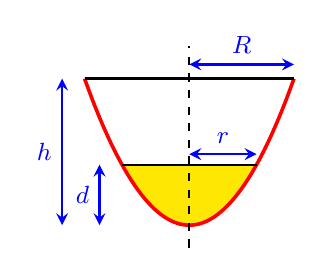
\begin{tikzpicture}[scale=0.95, >=stealth]
  % Miền tô vàng lớp dưới (chiều cao d)
  \fill[yellow!90!orange] plot[domain=-0.9:0.9, smooth] (\x, {\x*\x}) -- (-0.9,0.81) -- cycle;
  
  % Đường cong Parabol
  \draw[line width=1.3pt, red] plot[domain=-1.4:1.4, smooth] (\x, {\x*\x});
  \draw[line width=1pt] (-1.4,1.96) -- (1.4,1.96);
  \draw[line width=0.8pt] (-0.9,0.81) -- (0.9,0.81);
  
  % Trục đối xứng
  \draw[dashed, line width=0.8pt] (0,-0.3) -- (0,2.4);
  
  % Bán kính R và r
  \draw[<->, blue, line width=0.9pt] (0, 2.15) -- (1.4, 2.15) node[midway, above, font=\small] {$R$};
  \draw[<->, blue, line width=0.9pt] (0, 0.95) -- (0.9, 0.95) node[midway, above, font=\small] {$r$};
  
  % Chiều cao h và d
  \draw[<->, blue, line width=0.9pt] (-1.7, 0) -- (-1.7, 1.96) node[midway, left, font=\small] {$h$};
  \draw[<->, blue, line width=0.9pt] (-1.2, 0) -- (-1.2, 0.81) node[midway, left, font=\small] {$d$};
\end{tikzpicture}
\end{minipage}
\hfill
\begin{minipage}{0.48\textwidth}
\centering
\[
\mathbf{\color{red} \frac{d}{h} = \left(\frac{r}{R}\right)^2 \implies \frac{S_1}{S} = \left(\frac{r}{R}\right)^3 = \sqrt{\left(\frac{d}{h}\right)^3}}
\]
\end{minipage}
\end{tcolorbox}
\vspace{0.6cm}
\subsection*{\color{myblue}{d.2) Thể tích chảo parabol}}
\begin{tcolorbox}[colback=lightblue, colframe=myblue, arc=2mm]
\begin{minipage}{0.55\textwidth}
\centering
\vspace{0.5cm}
\begin{tcolorbox}[colback=white, colframe=black, sharp corners, boxrule=0.8pt]
\[
\mathbf{V = \frac{1}{2} \pi R^2 h}
\]
\end{tcolorbox}
\end{minipage}
\hfill
\begin{minipage}{0.4\textwidth}
\centering
% Hình 3: Chảo Parabol 3D
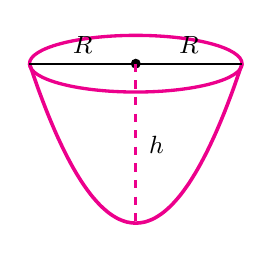
\begin{tikzpicture}[scale=0.9, >=stealth]
  % Vỏ chảo Parabol
  \draw[line width=1.3pt, magenta] plot[domain=-1.5:1.5, smooth] (\x, {\x*\x});
  \draw[line width=1.2pt, magenta] (0,2.25) ellipse (1.5cm and 0.4cm);
  
  % Tâm miệng chảo
  \fill (0,2.25) circle (2pt);
  
  % Bán kính R hai bên
  \draw[line width=0.8pt] (-1.5,2.25) -- (1.5,2.25);
  \node[above, font=\small\bfseries] at (-0.75, 2.25) {$R$};
  \node[above, font=\small\bfseries] at (0.75, 2.25) {$R$};
  
  % Đường cao h
  \draw[dashed, magenta, line width=1pt] (0,2.25) -- (0,0);
  \node[right, font=\small\bfseries] at (0.05, 1.1) {$h$};
\end{tikzpicture}
\end{minipage}
\end{tcolorbox}
\end{document}